\section{イントロダクション}

本資料は2025年に大谷・末原研究室(仮名)\footnote{
これまで森・大谷研究室と呼んでいたので筆者には少し違和感があるが、時期慣れるだろう。
}に入る学生が少しでも早く研究室に慣れるために用意した。大谷・末原研の研究室メンバーや研究内容に関して紹介する。なお基本的にこの冊子において教員・学生の人権はないが、それはこの冊子内でのみ通用するので注意すること。
%% の中でのみ通用すると思って欲しい。

\section{プロジェクト紹介}

\subsection{ILC計画}
aaa

\subsection{US-Japanカロリメータ開発}
aaa

\subsection{MEG~II実験}

MEG~II実験は$\mu^{+}\rightarrow e^{+}\gamma$と呼ばれるミューオンの稀な崩壊事象を探索する実験であり、スイス・ポールシェラー研究所(PSI)でデータ取得が行われている。$\mu^{+}\rightarrow e^{+}\gamma$は荷電レプトンフレーバーを破る崩壊事象であるが、SUSY-GUTによるとその崩壊分岐比は$\mathcal{O}(10^{-13})-\mathcal{O}(10^{-14})$と予測され、MEG~II実験では2021-2026年のデータ取得により感度$6\times10^{-14}$で$\mu^{+}\rightarrow e^{+}\gamma$探索を目指している。$\mu^{+}\rightarrow e^{+}\gamma$が発見されれば標準模型を超える新物理の決定的な証拠となり、発見されない場合でも新物理モデルに大きな制限を課すことになる。

\begin{figure}[h]
  \centering
  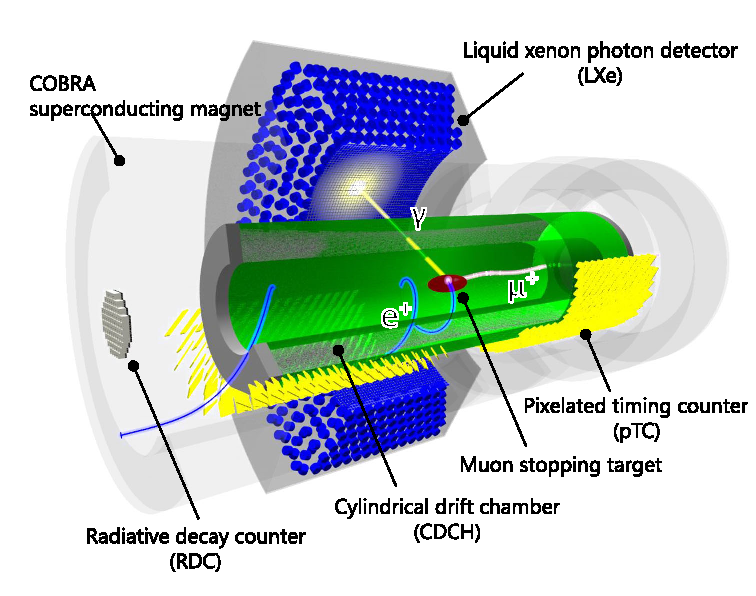
\includegraphics[width=0.6\columnwidth ,clip]{fig/MEGIIDetector.pdf}
  \caption{MEG~II実験検出器\cite{Baldini2018}}
  \label{fig:MEGIIDetector}
\end{figure}

MEG~II実験検出器を図~\ref{fig:MEGIIDetector}に示す。MEG~II実験検出器は陽電子とガンマ線検出に特化した検出器であり、陽電子検出はCDCH(Cylindrical Drift CHamber)とpTC(pixelated Timing Counter)、ガンマ線検出は液体キセノン(LXe)検出器でそれぞれ行われる。CDCHで陽電子のトラッキング、pTCでその時間を測定する。またLXe検出器でガンマ線の相互作用点の位置・時間、およびエネルギーを測定する。

  大谷・末原研では主にLXe検出器の運用・解析に注力しているが、例えば大矢さんは陽電子の解析に精通しているし、李さんはpTCの運用に携わるなど他の検出器をやっている教員・学生もいる。一応LXe検出器に携わる教員・学生を挙げると岩本さん、Lukas、潘さん、山本さん、馬越がいる。

  余談だが図~\ref{fig:MEGIIDetector}のCOBRA超伝導電磁石は検出器に勾配磁場をかけて低運動量陽電子を掃き出すために用いられるが、COBRAは20年前に大谷さんがデザインしたものであるから、「COBRAについて教えてください!」と大谷さんに言うと喜んで教えてくれるはずだ。PSIの大谷さんのデスクにはCOBRAを日本からスイスに海上輸送する際に使用されたと思われるステッカーが大切そうに飾られている。COBRAを愛してやまないようだ。

\subsection{次世代$\mu^{+}\rightarrow e^{+}\gamma$探索実験}
aaa

\subsection{PIONEER実験}
aaa

\section{メンバー紹介}
aaa

\subsection{大谷航准教授}
研究室のボス。優しい顔をしているが実際に優しい。困った学生がいると助けずにはいられない性格で、勤勉すぎていつも眠そうだ(図~\ref{fig:wataru_sleeping})。西口氏(図~\ref{fig:wataru})によると大谷さんの奥さんは恵子という名前で、大谷さんから「けいたん」と呼ばれているらしい。一方大谷さんはけいたんから「わたちゃん」と呼ばれているらしい。夫婦ともに仲睦まじくて微笑ましい。大谷さんは西口さん、身内さん\footnote{
身内賢太郎。神戸大素粒子実験グループの研究者。ダークマター探索を主にやっている、
}などから「わたぞう」と呼ばれているらしいが、これは彼が今は無き東大箕輪研に学生として所属していたときの愛称である。なんでも箕輪研では全学生にニックネームをつけていたらしい。今度大谷さんに会ったときに「わたぞう、けいたん元気?」と聞いてみよう。見たことのないような苦々しい顔を拝めるはずである。


\begin{wrapfigure}{R}{0.3\columnwidth}
  \vspace*{-\intextsep}
  \centering
  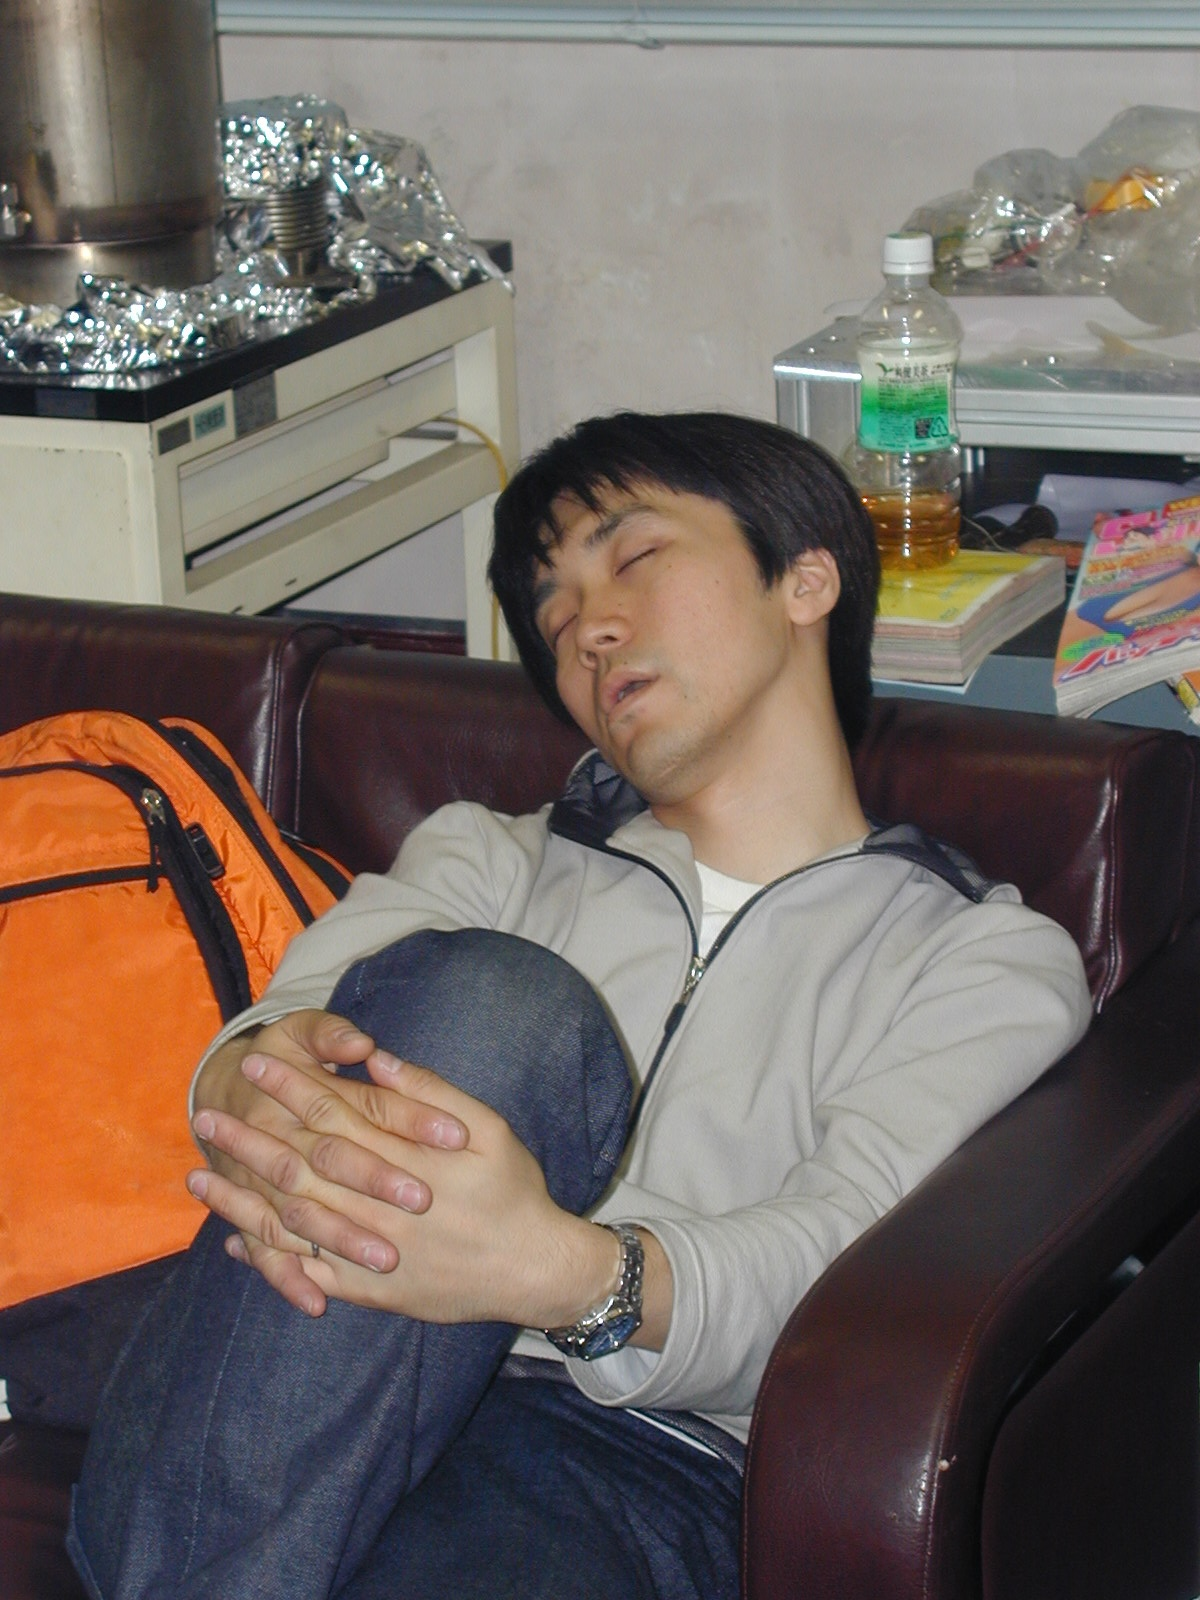
\includegraphics[width=0.3\columnwidth]{fig/wataru_sleeping.jpg}
  \caption{研究で疲れ果てて仮眠を取る若かりし頃の大谷さん。当時から研究のやり過ぎで寝不足だったようである。}
  \label{fig:wataru_sleeping}
\end{wrapfigure}

\begin{figure}[h]
  \centering
  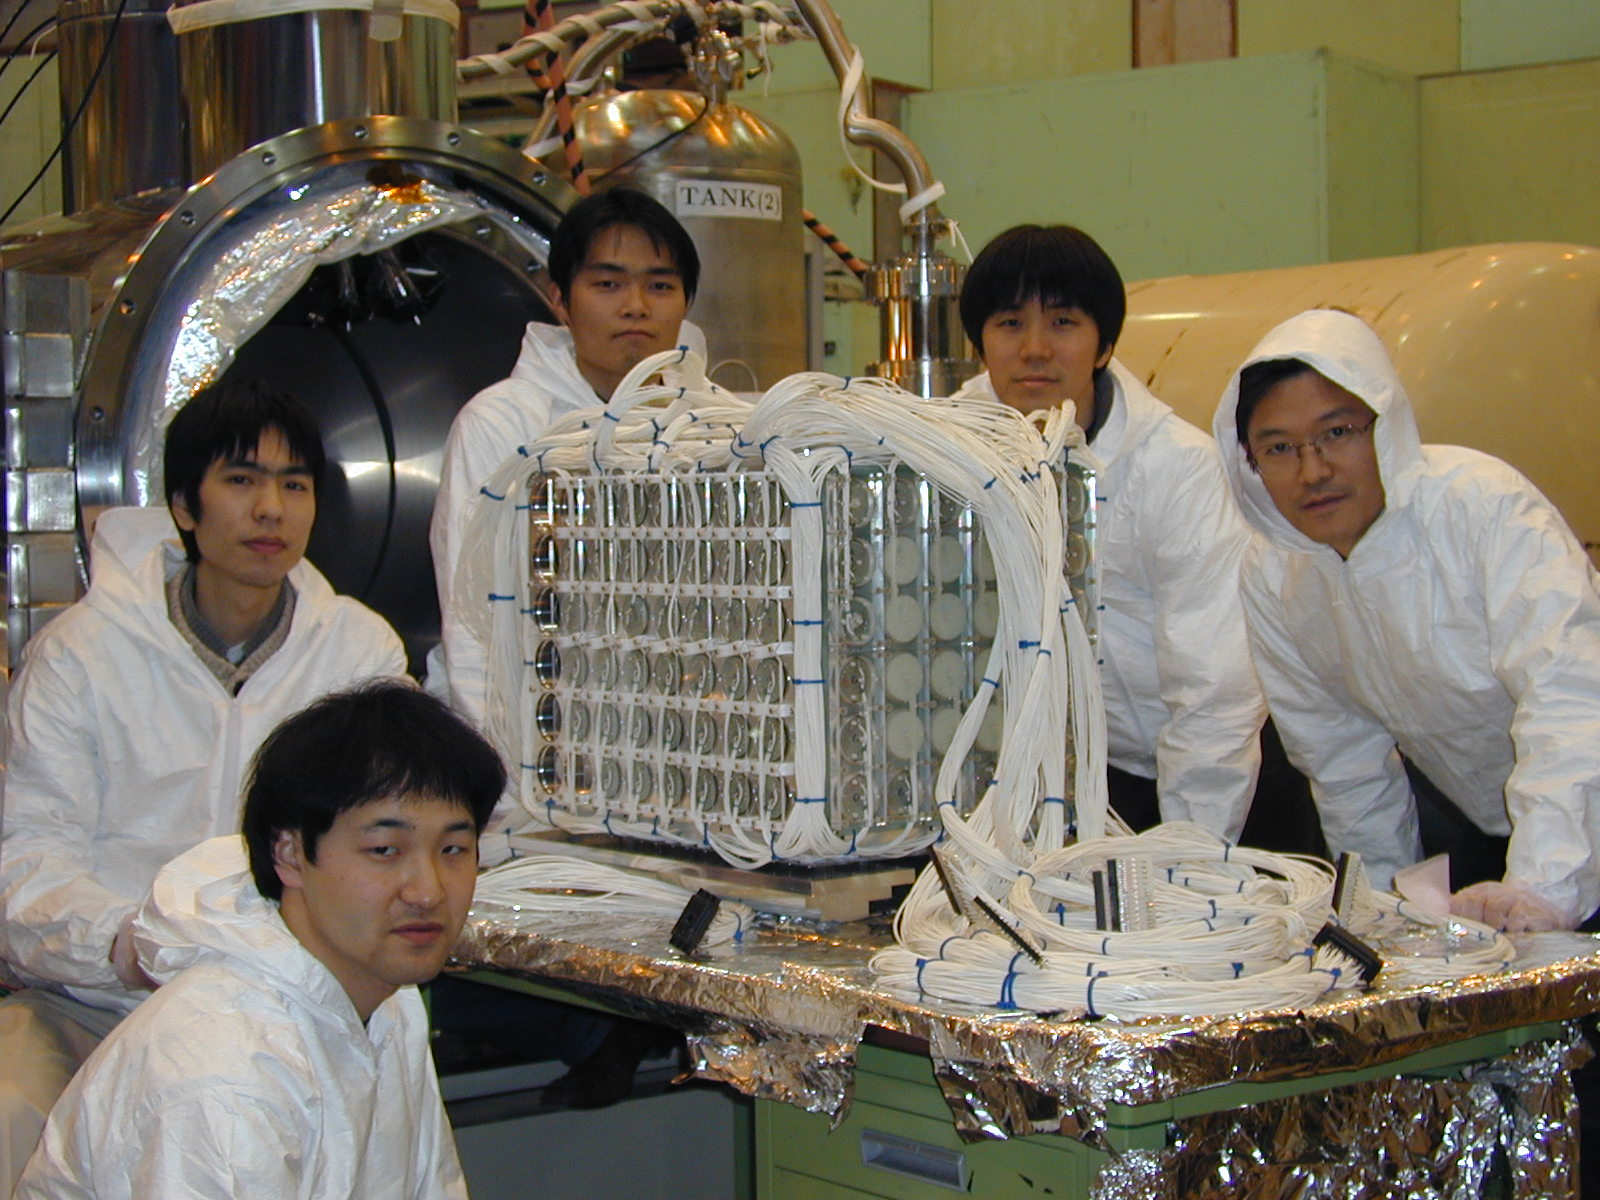
\includegraphics[width=0.7\columnwidth,clip]{fig/wataru.jpg}
  \caption{Large prototypeと呼ばれるMEG II液体キセノン検出器の試作器を試験する大谷さんたち。右から反時計回りに三原智さん、大谷さん、西口??さん、澤田龍さん、あと名前わからない人。三原さんと西口さんは現在KEKの研究者で、澤田さんは(ご存知の通り)ICEPPの研究者である。彼らは若いころキセノン検出器の開発をしていた。}
  \label{fig:wataru}
\end{figure}


\subsection{末原大幹特任准教授}
aaa




\subsection{岩本敏幸助教}

MEG~IIのランコーディネータ。MEG~IIに関わらない限り会う機会はゼロに近いが、一旦MEG~IIに手を出したらひょっとすると大谷さんよりお世話になるかもしれない。なぜなら基本的に彼はPSIに常駐しており学生の研究・生活両方の面倒を見ているからだ。酒豪であることが知られているためお酒を渡すと満面の笑みを見せてくれる。「今度の飲み会で飲もう」と言う岩本さんの声が聞こえてくる。PSIの岩本さんのデスク後ろの棚には日本酒が常備されている。



\subsection{Lukas Gerritzen特任助教}

気のいいドイツ人。いつもニコニコ笑っており、世話好きなお兄さんといった感じ。彼にドイツ語で話しかけると試すように少し難しいドイツ語が返ってくる。筆者はアルプス山麓のPradenにある彼の彼女の別荘に連れて行ってもらったことがあるが、絶景だった(図~\ref{})。お返しに私の実家の島にあるお寿司屋さんに連れて行ってあげると、嬉しそうに中指を立ててくれた(図~\ref{})。これがツンデレな彼なりの感謝を伝える唯一の方法なのだと筆者は思うようにしている(もしかしたらベジタリアンの彼と彼の彼女に魚を食べさせた私に対する当てつけなのかもしれないが、気のせいだろう)。



今年6月にSBB(スイス連邦鉄道)関連のソフトウェア系企業に就職予定であるが、彼の更なる活躍に期待しよう。

\subsection{潘晟特任助教}

MEG~IIキセノン検出器のエキスパート。特に実機の運用に関して彼の右に出る人は(岩本さんをおいて)いないだろう。彼が博士課程の学生のときすでに息子(図~\ref{})がいたという強烈エピソードを持つ(主観)。またPSIから片道10 kmはあるKauflandと呼ばれるドイツのスーパーまで歩いて買い出しに行くらしく、かなりの体力の持ち主である。


\subsection{大矢淳史特任助教}

MEG~IIの解析リーダー。解析のことならなんでも知っているのではないか、と筆者は思っている。365日物理をやっているような人で、どのような話題に対しても二言目には物理のことを話している。強い思想の持ち主で、時々「やばい」と筆者は個人的に思っているが、その思想に共感するかどうかは人それぞれである。%% どうあれ、強い思想を持っていると言うことでは皆一致している。
研究のことでテキトウなことを言ってしまうとすぐに鋭いカウンターが返ってくるから、彼の前では優等生のように理路整然と話そう。ちなみにmod13%% \ref{subsec:mod13}
と呼ばれるゲームが大好きなので「mod13ってなんですか?教えてください!」と言えば喜んで教えてくれること間違いない。
%% 大矢さんの逆鱗に触れないよう気をつけよう。研究のことでテキトウなことを言ってしまうとすぐに鋭いカウンターが返って

\begin{wrapfigure}{R}{0.3\columnwidth}
  \vspace*{-\intextsep}
  \centering
  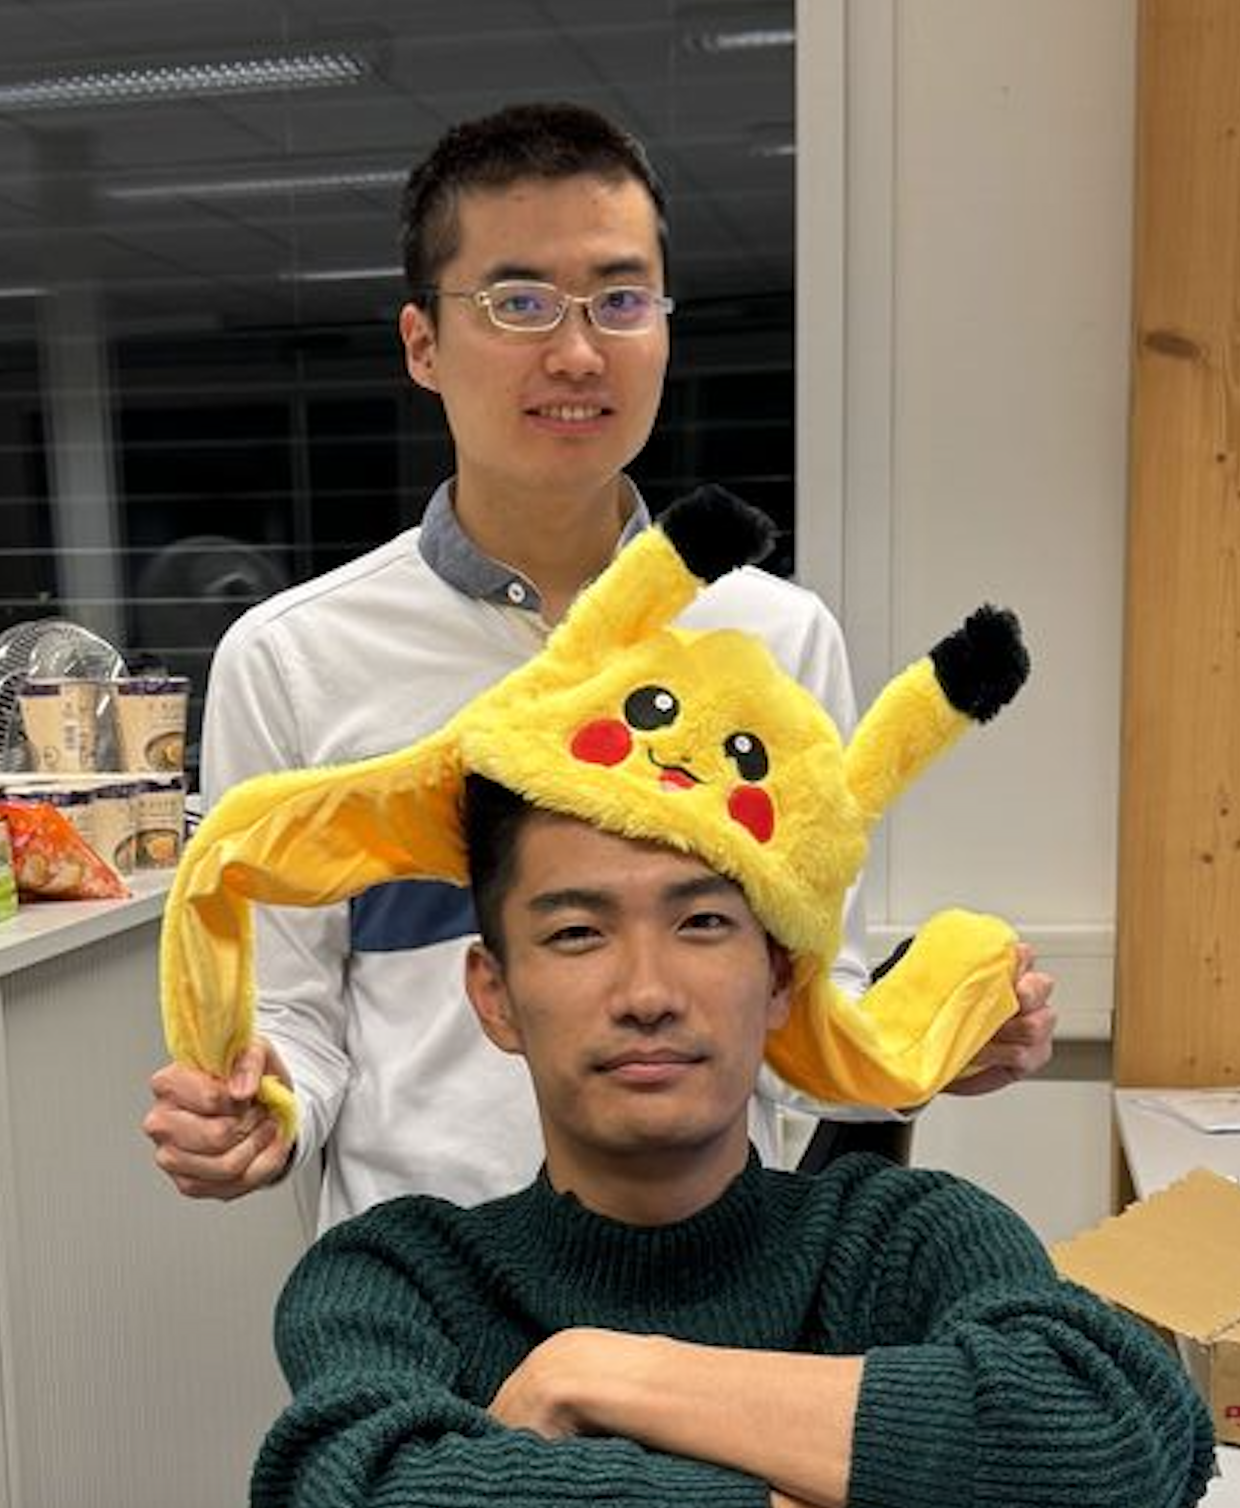
\includegraphics[width=0.3\columnwidth]{fig/atsushi_kensuke.png}
  \caption{解析の間違いに気づいて落ち込む山本さんとそれに同情する大谷さん。山本さんが被っているピカチュウはスイスのOktober Festivalで買ったもの。みんなのお気に入り。}
  \label{fig:atsushi_kensuke}
\end{wrapfigure}

\subsection{山本健介(D4)}

MEG~IIキセノン検出器の解析マン。基本的にエピソードに事欠かないが、例えば大学3年で飛び級してICEPPに来たとか、大学院入学後マーチングバンドの修行のために3ヶ月アメリカに留学するなど盛りだくさんである。大変な努力家で努力に比例して夜酒は増えているとか(未確認)。特任助教に内定しており、博士号取得後すぐに着任予定である。引き続きMEG~II解析の実働部隊として活躍が期待されている。%% 博士課程でMEG~II解析に注力する筆者にとって頼れる先輩である。


\subsection{村田樹(D4)}
aaa

\subsection{池田史(D3)}
aaa

\subsection{李維遠(D2)}
\label{subsec:weiyuan}
aaa

\subsection{小川拓泰(D1)}
aaa

\subsection{神山大樹(D1)}
aaa

\subsection{高津大誠(D1)}
aaa

\subsection{馬越隆成(D1)}
aaa

\subsection{榊原澪(M2)}

MEG~III関連のビームテスト、シミュレーションでその手腕を振るっている。かなりのやり手で、筆者はいつも下を巻いている。ワイン好きで「両親ともお酒強いんで(私も強いです)」と言いながらごくごくとワインを飲み干してしまう。%% 彼女もまた隠れ酒豪である。
ゲーマーであり暇を見つけては少しずつゲームを進めているらしい。

\begin{wrapfigure}{R}{0.3\columnwidth}
  \vspace*{-\intextsep}
  \centering
  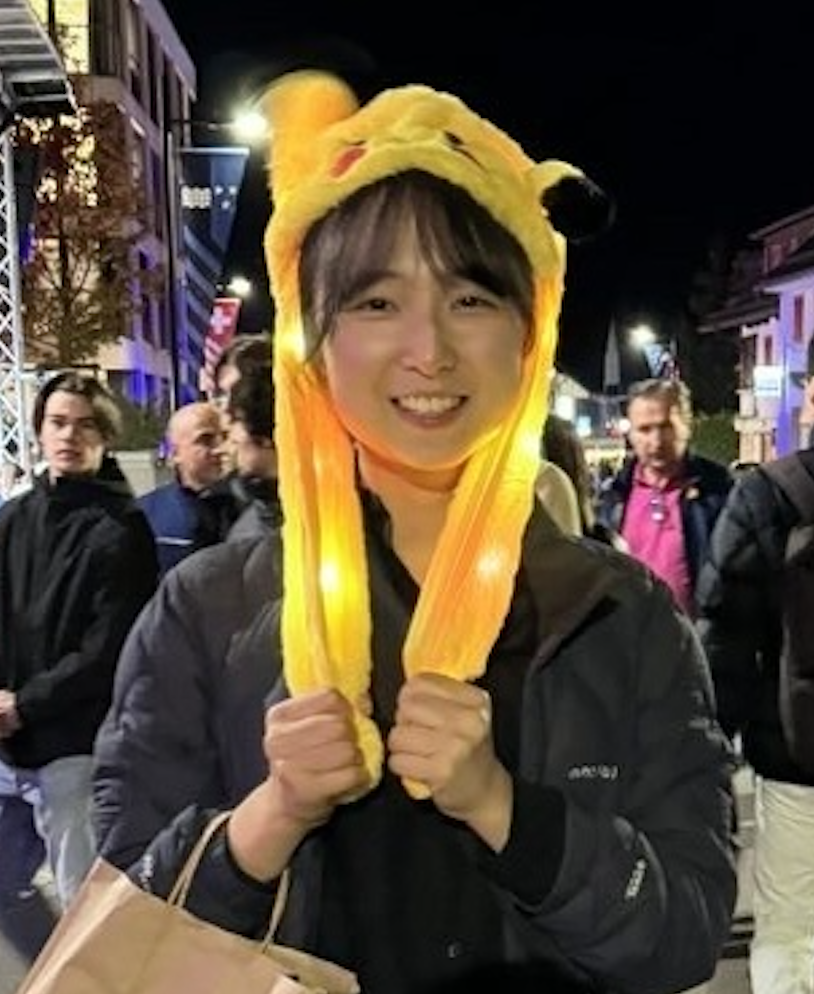
\includegraphics[width=0.3\columnwidth]{fig/rei.png}
  \caption{榊原さん。Oktober Festivalに行ったときに撮られた。頭にはピカチュウ(純正!)を被っている。}
  \label{fig:rei}
\end{wrapfigure}

\subsection{清野拓己(M2)}
ILC関連のラボ実験・解析に熱心に取り組んでいる。かと思えばPIONEER向けの光センサーの性能評価試験をするなど割と頼めばなんでもやってくれそう。PSIにインターンで来た際、数々の伝説を残した。Lauterbrunenと呼ばれる観光名所に行く電車の中でゲイのAI研究者と仲良くなり、一緒に旅行中に「You are cute.」と言い寄られ、咄嗟に「I love woman.」と断ると「I respect you.」という珍妙な返事をいただいたことがあるらしい。またPSIのカフェテリアでおかわりをしまくったせいで顔を覚えられてしまい、最終的におかわり禁止を言い渡されたなど枚挙にいとまがない。なおおかわり禁止は彼の帰国の前日だったので彼はまんまと逃げおおせてしまった。

\begin{wrapfigure}{R}{0.3\columnwidth}
  \vspace*{-\intextsep}
  \centering
  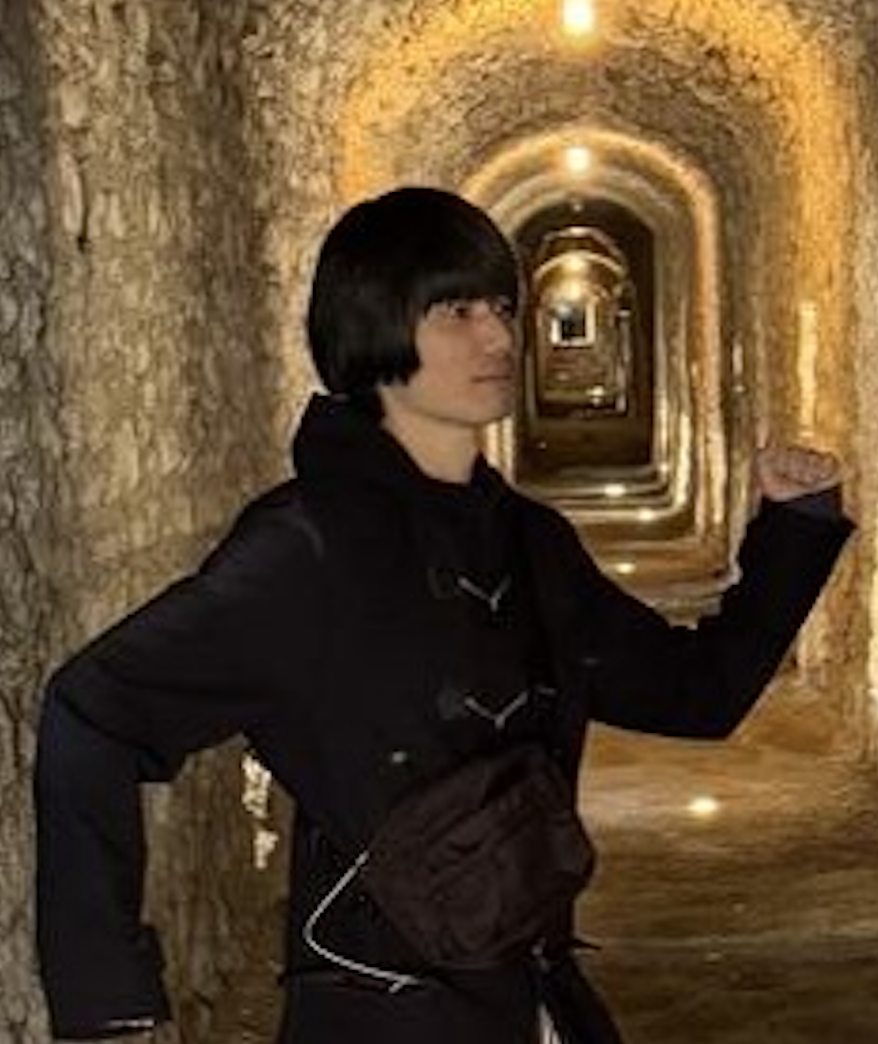
\includegraphics[width=0.3\columnwidth]{fig/takumi.png}
  \caption{清野くん。Bellinzonaにあるお城のMurataの中に入ったときに撮られた。}
  \label{fig:takumi}
\end{wrapfigure}

\section{その他}

\subsection{MEG-J Wiki}

大谷・末原研には過去の先輩から引き継ぎ、加筆し続けられているwikiページが存在する。その名を\href{http://meg.icepp.s.u-tokyo.ac.jp/restricted/dokuwiki/doku.php?id=start}{MEG-J Wiki}と言うが、とても大切なこと(例えば解析ソフトのインストール方法や大学院生活の身の処し方など)が至る所に書かれているから暇なときに覗いてみよう。

\subsection{Mod13}
\label{subsec:mod13}
大谷・末原研にはmod13と呼ばれる悪魔のゲームがある(主観)。このゲームは大矢さんが研究室に持ち込んだもので、大矢さんは高校時代に友人から教わったらしい。トランプを使って行われるが、詳しくは\href{http://meg.icepp.s.u-tokyo.ac.jp/restricted/dokuwiki/doku.php?id=start}{MEG-J WikiのMiscellanious}を参照のこと。簡単に言うと大矢さんが勝って気持ちよくなるためのゲーム。

\subsection{Jopi}

PSIにはJopiと呼ばれるかわいらしい猫が住んでいる(図~\ref{fig:jopi})。とても人懐っこく、よく「ニャーニャー」と鳴きながら近づいてくる。研究で疲れ果てた研究者のメンタルサポーターであり、PSIにはJopiの密かなファンがたくさんいる。

\begin{wrapfigure}{R}{0.3\columnwidth}
  \vspace*{-\intextsep}
  \centering
  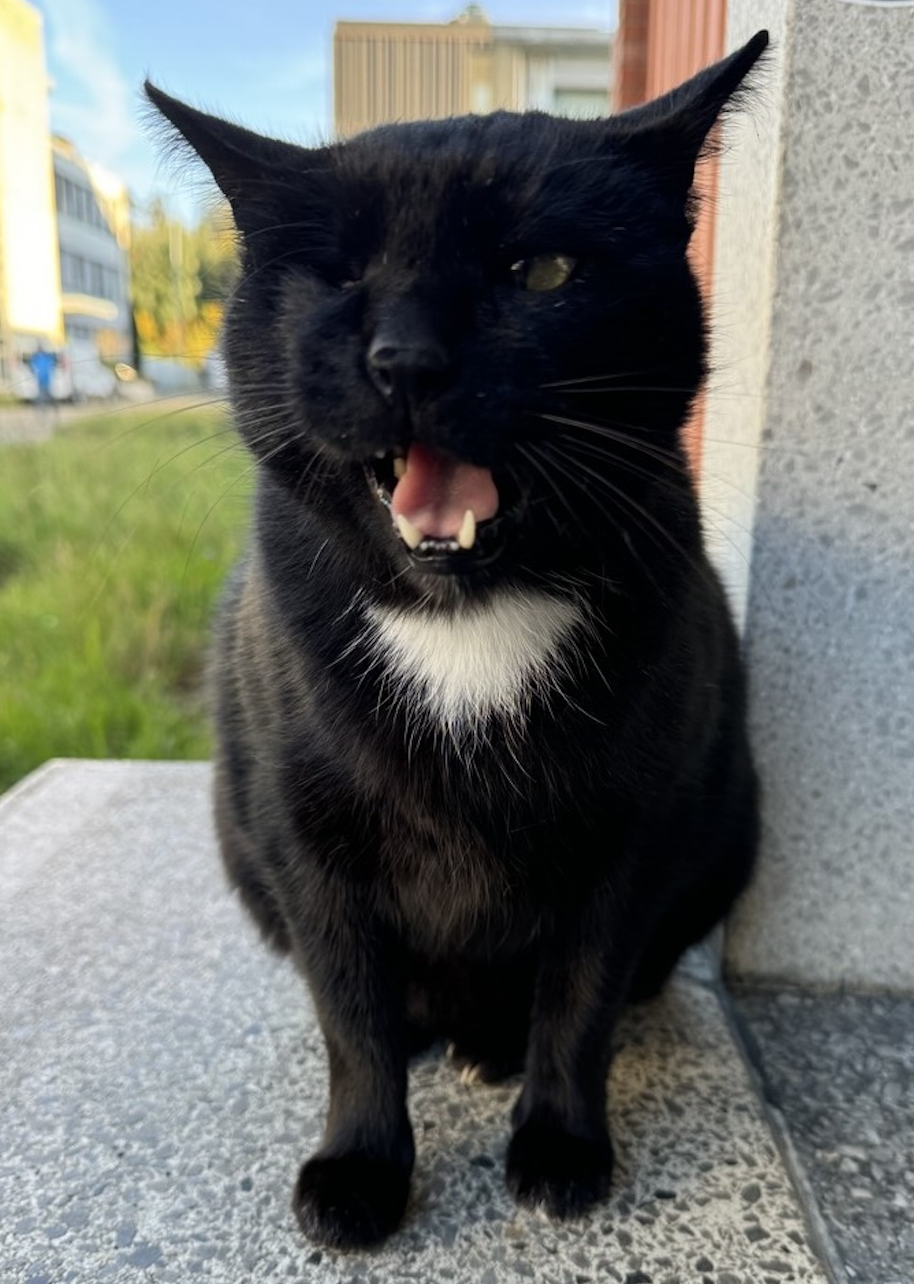
\includegraphics[width=0.3\columnwidth]{fig/jopi.png}
  \caption{Jopi。PSIに住む黒猫。人懐っこくてよく喋る。みんなから愛されていて家もある。}
  \label{fig:jopi}
\end{wrapfigure}
